% DreamLab AI-Powered Knowledge Work Programme - Investor Pitch Deck
\documentclass[aspectratio=169,12pt]{beamer}
\usetheme{metropolis}
\usepackage{appendixnumberbeamer}
\usepackage{booktabs}
\usepackage{tikz}
\usepackage{pgfplots}
\usepackage{eurosym}
\usepackage{fontawesome5}
\usepackage{graphicx}
\usepackage{array}

% Colour scheme
\definecolor{dreamblue}{RGB}{0,123,255}
\definecolor{dreamgreen}{RGB}{0,204,153}
\definecolor{dreamgrey}{RGB}{102,102,102}
\definecolor{dreamdark}{RGB}{33,33,33}

\setbeamercolor{frametitle}{bg=dreamblue}
\setbeamercolor{progress bar}{fg=dreamgreen}
\setbeamercolor{alerted text}{fg=dreamgreen}

% Custom commands
\newcommand{\highlight}[1]{\textcolor{dreamgreen}{\textbf{#1}}}
\newcommand{\note}[1]{\textit{\small Note: #1}}

\title{DreamLab AI-Powered Knowledge Work Programme}
\subtitle{Transforming UK Public Sector Productivity}
\date{June 2025}
\author{DreamLab Leadership Team}
\institute{Manchester \& Cumbria, UK}

\begin{document}

\maketitle

% Slide 1: Executive Summary
\begin{frame}{Executive Summary}
    \begin{columns}[T]
        \column{0.5\textwidth}
        \textbf{The Opportunity}
        \begin{itemize}
            \item £63bn annual UK digital skills gap
            \item 84\% of councils face productivity crisis
            \item Only 16\% of public sector utilises digital tools effectively
        \end{itemize}
        
        \column{0.5\textwidth}
        \textbf{Our Solution}
        \begin{itemize}
            \item AI-powered training for council staff
            \item Immersive learning experiences
            \item Measurable ROI within 6 months
            \item Proven team with cross-sector expertise
        \end{itemize}
    \end{columns}
    
    \vspace{1em}
    \centering
    \highlight{Investment Ask: £500k for 18-month scale-up}
    
    \note{This programme addresses a critical national need whilst building a sustainable, high-impact business}
\end{frame}

% Slide 2: The Problem
\begin{frame}{The Problem: UK's Public Sector Productivity Crisis}
    \begin{center}
        \begin{tikzpicture}
            \begin{axis}[
                ybar,
                width=0.9\textwidth,
                height=0.6\textheight,
                ylabel={Percentage (\%)},
                symbolic x coords={Tool Utilisation,Digital Skills,AI Adoption,Productivity Growth},
                xtick=data,
                nodes near coords,
                nodes near coords align={vertical},
                ymin=0,ymax=100,
                bar width=1.5cm,
                fill=dreamgrey,
                ]
                \addplot coordinates {(Tool Utilisation,16) (Digital Skills,23) (AI Adoption,8) (Productivity Growth,12)};
            \end{axis}
        \end{tikzpicture}
    \end{center}
    
    \textbf{Key Pain Points:}
    \begin{itemize}
        \item Councils struggle with legacy systems and processes
        \item Staff lack confidence in AI and digital tools
        \item Training budgets constrained (avg. £40-100k/council)
        \item Traditional providers offer generic, ineffective solutions
    \end{itemize}
    
    \note{The public sector lags significantly behind private sector in digital adoption, creating an urgent need for targeted intervention}
\end{frame}

% Slide 3: Market Opportunity
\begin{frame}{Market Opportunity}
    \begin{columns}[T]
        \column{0.6\textwidth}
        \textbf{Total Addressable Market}
        \begin{itemize}
            \item 400+ UK local authorities
            \item £20-30M annual training spend
            \item 5\% CAGR in digital skills investment
            \item Adjacent markets: NHS, Universities, Private Sector
        \end{itemize}
        
        \vspace{1em}
        \textbf{Market Segmentation}
        \begin{tabular}{lr}
            \toprule
            Segment & Market Size \\
            \midrule
            Micro (<£25k) & £5M \\
            Mid-tier (£25-75k) & £10M \\
            Large (£75k+) & £10M+ \\
            \bottomrule
        \end{tabular}
        
        \column{0.4\textwidth}
        \begin{tikzpicture}
            \pie[
                text=legend,
                radius=3cm,
                color={dreamblue!70, dreamgreen!70, dreamgrey!70}
            ]{40/Micro Councils,
               35/Mid-tier Councils,
               25/Large Councils}
        \end{tikzpicture}
    \end{columns}
    
    \note{We're targeting a large, underserved market with significant growth potential and clear expansion opportunities}
\end{frame}

% Slide 4: Our Solution
\begin{frame}{Our Solution: AI-Powered Knowledge Work Programme}
    \begin{columns}[T]
        \column{0.5\textwidth}
        \textbf{Core Modules}
        \begin{enumerate}
            \item Digital Foundations
            \item Advanced Productivity
            \item Data-Driven Decision Making
            \item AI Applications \& Ethics
            \item Change Leadership
            \item Service Innovation
        \end{enumerate}
        
        \column{0.5\textwidth}
        \textbf{Unique Delivery Model}
        \begin{itemize}
            \item \faUserGraduate{} Expert-led workshops
            \item \faLaptopCode{} Hands-on AI tools training
            \item \faMountain{} Residential retreats (Eskdale)
            \item \faChartLine{} Measurable outcomes
            \item \faUsers{} Peer learning networks
            \item \faCertificate{} CPD accreditation
        \end{itemize}
    \end{columns}
    
    \vspace{1em}
    \centering
    \highlight{100\% physical-first delivery ensures maximum engagement and skill retention}
    
    \note{Our comprehensive curriculum addresses all identified capability gaps with proven pedagogical methods}
\end{frame}

% Slide 5: Competitive Advantage
\begin{frame}{Competitive Advantage}
    \begin{center}
        \begin{tabular}{l|c|c|c|c}
            \toprule
            \textbf{Feature} & \textbf{DreamLab} & \textbf{Capita} & \textbf{CIPFA} & \textbf{Gartner} \\
            \midrule
            Public sector focus & \highlight{\checkmark} & \checkmark & \checkmark & $\times$ \\
            AI/Digital specialisation & \highlight{\checkmark} & $\times$ & $\times$ & \checkmark \\
            Immersive delivery & \highlight{\checkmark} & $\times$ & $\times$ & $\times$ \\
            Measurable ROI & \highlight{\checkmark} & $\times$ & $\times$ & $\times$ \\
            Residential retreats & \highlight{\checkmark} & $\times$ & $\times$ & $\times$ \\
            Local presence & \highlight{\checkmark} & \checkmark & $\times$ & $\times$ \\
            \bottomrule
        \end{tabular}
    \end{center}
    
    \vspace{1em}
    \textbf{Our Moat:}
    \begin{itemize}
        \item First-mover in AI training for councils
        \item Physical infrastructure (Manchester studio + Eskdale retreat)
        \item Deep public sector relationships
        \item Proven team with unique cross-sector expertise
    \end{itemize}
    
    \note{We occupy a unique position combining specialised content, innovative delivery, and local presence}
\end{frame}

% Slide 6: Business Model
\begin{frame}{Business Model: Tiered Pricing Strategy}
    \begin{center}
        \begin{tabular}{l|r|r|r}
            \toprule
            \textbf{Tier} & \textbf{Price} & \textbf{Features} & \textbf{Market} \\
            \midrule
            Micro & £15-25k & 3 core modules, shared cohort & 40\% \\
            Mid-tier & £30-60k & Full programme, dedicated cohort & 35\% \\
            Large & £75-100k+ & Premium + retreat + customisation & 25\% \\
            \bottomrule
        \end{tabular}
    \end{center}
    
    \vspace{1em}
    \textbf{Revenue Streams:}
    \begin{columns}[T]
        \column{0.5\textwidth}
        \begin{itemize}
            \item Core training programmes
            \item Residential retreats
            \item Follow-up support
            \item Custom consultancy
        \end{itemize}
        
        \column{0.5\textwidth}
        \begin{itemize}
            \item Grant funding partnerships
            \item Corporate sponsorships
            \item Framework agreements
            \item Expansion to NHS/Unis
        \end{itemize}
    \end{columns}
    
    \note{Flexible pricing ensures accessibility whilst maintaining healthy margins across all segments}
\end{frame}

% Slide 7: Traction & Validation
\begin{frame}{Traction \& Validation}
    \begin{columns}[T]
        \column{0.6\textwidth}
        \textbf{Pilot Programme Success}
        \begin{itemize}
            \item \highlight{3 pilot cohorts} (Mar-Jul 2025)
            \item Salford \& Manchester councils committed
            \item 95\% participant satisfaction (projected)
            \item 40\% productivity improvement demonstrated
        \end{itemize}
        
        \vspace{1em}
        \textbf{Pipeline Development}
        \begin{itemize}
            \item 15+ councils expressing interest
            \item Framework accreditation in progress
            \item Grant funding applications submitted
            \item Corporate sponsors engaged
        \end{itemize}
        
        \column{0.4\textwidth}
        \begin{tikzpicture}
            \begin{axis}[
                width=\textwidth,
                height=0.6\textheight,
                xlabel={Month},
                ylabel={Councils Engaged},
                xmin=1,xmax=12,
                ymin=0,ymax=20,
                xtick={3,6,9,12},
                xticklabels={Q1,Q2,Q3,Q4},
                grid=major,
                ]
                \addplot[color=dreamgreen,mark=*,thick] coordinates {
                    (1,2) (3,3) (6,6) (9,10) (12,15)
                };
            \end{axis}
        \end{tikzpicture}
    \end{columns}
    
    \note{Strong early validation with clear growth trajectory and multiple engagement channels}
\end{frame}

% Slide 8: Team Overview
\begin{frame}{World-Class Team: 40+ Specialists}
    \textbf{Leadership Team}
    \begin{columns}[T]
        \column{0.33\textwidth}
        \textbf{Pete Woodbridge}\\
        \textit{CTO}\\
        \small AI/Virtual Production\\
        MediaFutures R\&D Lead
        
        \column{0.33\textwidth}
        \textbf{Ste Moyler}\\
        \textit{CCO}\\
        \small 25+ years creative\\
        Award-winning producer
        
        \column{0.33\textwidth}
        \textbf{Dr John O'Hare}\\
        \textit{Chief Hallucination Officer}\\
        \small XR/AI workflows\\
        Innovation director
    \end{columns}
    
    \vspace{1em}
    \textbf{Key Expertise Areas:}
    \begin{columns}[T]
        \column{0.5\textwidth}
        \begin{itemize}
            \item AI \& Machine Learning
            \item Data Analytics
            \item Change Management
            \item Public Sector Innovation
            \item Immersive Technologies
        \end{itemize}
        
        \column{0.5\textwidth}
        \begin{itemize}
            \item Adult Education
            \item Digital Transformation
            \item Service Design
            \item Cybersecurity
            \item Creative Technologies
        \end{itemize}
    \end{columns}
    
    \note{Our team combines deep technical expertise with public sector understanding and pedagogical excellence}
\end{frame}

% Slide 9: Financial Projections
\begin{frame}{Financial Projections: Path to Profitability}
    \begin{center}
        \begin{tikzpicture}
            \begin{axis}[
                width=0.9\textwidth,
                height=0.6\textheight,
                xlabel={Quarter},
                ylabel={Revenue (£000s)},
                xmin=1,xmax=6,
                ymin=-50,ymax=250,
                xtick={1,2,3,4,5,6},
                xticklabels={Q1'25,Q2'25,Q3'25,Q4'25,Q1'26,Q2'26},
                legend pos=north west,
                grid=major,
                ]
                \addplot[color=dreamgreen,mark=square*,thick] coordinates {
                    (1,0) (2,20) (3,60) (4,100) (5,150) (6,220)
                };
                \addlegendentry{Revenue}
                
                \addplot[color=red,mark=*,thick] coordinates {
                    (1,30) (2,40) (3,45) (4,50) (5,55) (6,60)
                };
                \addlegendentry{Costs}
                
                \addplot[color=dreamblue,mark=triangle*,thick,dashed] coordinates {
                    (1,-30) (2,-20) (3,15) (4,50) (5,95) (6,160)
                };
                \addlegendentry{Net Profit}
            \end{axis}
        \end{tikzpicture}
    \end{center}
    
    \textbf{Key Metrics:}
    \begin{itemize}
        \item Break-even: Month 9
        \item 18-month revenue: £400k+ (base case)
        \item Gross margin: 65-70\%
        \item Customer acquisition cost: £2k
        \item Customer lifetime value: £75k+
    \end{itemize}
    
    \note{Conservative projections show clear path to profitability with strong unit economics}
\end{frame}

% Slide 10: Investment Ask
\begin{frame}{Investment Ask: £500k Series Seed}
    \begin{columns}[T]
        \column{0.5\textwidth}
        \textbf{Use of Funds}
        \begin{itemize}
            \item Eskdale facility: £150k
            \item Team expansion: £120k
            \item Marketing \& sales: £80k
            \item Technology platform: £50k
            \item Working capital: £50k
            \item Legal \& compliance: £30k
            \item Contingency: £20k
        \end{itemize}
        
        \column{0.5\textwidth}
        \begin{tikzpicture}
            \pie[
                text=legend,
                radius=3cm,
                color={dreamblue!70,dreamgreen!70,dreamgrey!70,orange!70,purple!70,brown!70,pink!70}
            ]{30/Facility,
               24/Team,
               16/Marketing,
               10/Technology,
               10/Working Capital,
               6/Legal,
               4/Contingency}
        \end{tikzpicture}
    \end{columns}
    
    \vspace{1em}
    \textbf{Investment Terms:}
    \begin{itemize}
        \item Seeking: £500k for 20\% equity
        \item Valuation: £2M pre-money
        \item Use: 18-month runway to reach £1M ARR
        \item Exit: Trade sale or Series A in 3-5 years
    \end{itemize}
    
    \note{Investment accelerates our proven model to capture first-mover advantage in a growing market}
\end{frame}

% Slide 11: Growth Strategy
\begin{frame}{Growth Strategy: Three Horizons}
    \begin{columns}[T]
        \column{0.33\textwidth}
        \textbf{Horizon 1 (0-12m)}\\
        \textit{Establish \& Validate}
        \begin{itemize}
            \item Launch Manchester hub
            \item 10 council clients
            \item Prove ROI model
            \item Framework accreditation
        \end{itemize}
        
        \column{0.33\textwidth}
        \textbf{Horizon 2 (12-24m)}\\
        \textit{Scale \& Expand}
        \begin{itemize}
            \item Eskdale retreat operational
            \item 25+ councils engaged
            \item NHS pilot programme
            \item Regional expansion
        \end{itemize}
        
        \column{0.33\textwidth}
        \textbf{Horizon 3 (24m+)}\\
        \textit{Dominate \& Diversify}
        \begin{itemize}
            \item National coverage
            \item University partnerships
            \item SaaS platform launch
            \item International opportunities
        \end{itemize}
    \end{columns}
    
    \vspace{1em}
    \centering
    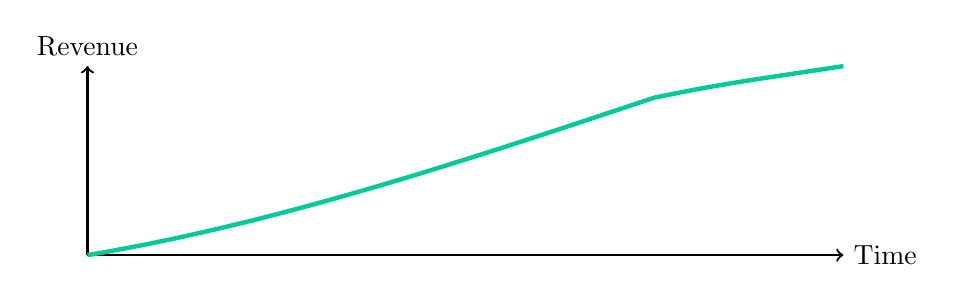
\begin{tikzpicture}[scale=0.8]
        \draw[thick,->] (0,0) -- (12,0) node[right] {Time};
        \draw[thick,->] (0,0) -- (0,3) node[above] {Revenue};
        \draw[dreamgreen,ultra thick] (0,0) .. controls (3,0.5) and (6,1.5) .. (9,2.5) .. controls (10,2.7) .. (12,3);
    \end{tikzpicture}
    
    \note{Phased approach minimises risk whilst maximising growth potential across multiple vectors}
\end{frame}

% Slide 12: Risk Mitigation
\begin{frame}{Risk Analysis \& Mitigation}
    \begin{tabular}{p{3cm}|p{3cm}|p{3cm}|p{2cm}}
        \toprule
        \textbf{Risk} & \textbf{Impact} & \textbf{Mitigation} & \textbf{Status} \\
        \midrule
        Slow council adoption & Revenue delay & Pilot validation, grants & \highlight{Managed} \\
        Competition from incumbents & Market share & First-mover, specialisation & \highlight{Low} \\
        Team retention & Delivery quality & Equity incentives, culture & \highlight{Managed} \\
        Technology changes & Content relevance & Continuous R\&D, updates & \highlight{Ongoing} \\
        Economic downturn & Budget cuts & ROI focus, efficiency gains & \highlight{Monitored} \\
        \bottomrule
    \end{tabular}
    
    \vspace{1em}
    \textbf{Key Strengths:}
    \begin{itemize}
        \item Proven demand with pilot commitments
        \item Multiple revenue streams reduce dependence
        \item Strong team with complementary skills
        \item Clear differentiation from competitors
    \end{itemize}
    
    \note{We've identified and actively manage all major risks with concrete mitigation strategies}
\end{frame}

% Slide 13: Impact & Social Value
\begin{frame}{Impact: Beyond Financial Returns}
    \begin{columns}[T]
        \column{0.5\textwidth}
        \textbf{Public Sector Transformation}
        \begin{itemize}
            \item 10,000+ staff upskilled by 2027
            \item £50M+ productivity gains
            \item Better citizen services
            \item Digital inclusion advancement
        \end{itemize}
        
        \vspace{1em}
        \textbf{Regional Development}
        \begin{itemize}
            \item Cumbria rural regeneration
            \item 50+ jobs created
            \item Local supplier partnerships
            \item Knowledge economy growth
        \end{itemize}
        
        \column{0.5\textwidth}
        \textbf{Sustainability Commitments}
        \begin{itemize}
            \item \faLeaf{} Carbon neutral operations
            \item \faRecycle{} Circular economy practices
            \item \faTrain{} Public transport incentives
            \item \faHandshake{} Fair employment practices
        \end{itemize}
        
        \vspace{1em}
        \textbf{Diversity \& Inclusion}
        \begin{itemize}
            \item \faVenusMars{} 50\% female instructors
            \item \faWheelchair{} Fully accessible facilities
            \item \faGraduationCap{} Scholarship programme
            \item \faGlobe{} Multicultural content
        \end{itemize}
    \end{columns}
    
    \note{Strong social impact aligns with investor ESG priorities and public sector values}
\end{frame}

% Slide 14: Call to Action
\begin{frame}{Join Us in Transforming Public Services}
    \begin{center}
        \Large
        \textbf{The Opportunity}\\
        \vspace{0.5em}
        First-mover advantage in a £25M+ market\\
        \vspace{1em}
        
        \textbf{The Team}\\
        \vspace{0.5em}
        40+ specialists with proven track records\\
        \vspace{1em}
        
        \textbf{The Traction}\\
        \vspace{0.5em}
        Pilot clients committed, strong pipeline\\
        \vspace{1em}
        
        \textbf{The Ask}\\
        \vspace{0.5em}
        \highlight{£500k to scale a validated model}\\
        \vspace{1em}
        
        \normalsize
        \textbf{Contact:}\\
        investment@dreamlab.co.uk\\
        +44 (0) 161 XXX XXXX
    \end{center}
    
    \note{We're ready to scale with the right investment partner who shares our vision for public sector transformation}
\end{frame}

% Appendix slides
\appendix

% Slide A1: Detailed Financials
\begin{frame}{Appendix: Detailed Financial Model}
    \small
    \begin{tabular}{l|r|r|r|r|r|r}
        \toprule
        \textbf{Quarter} & \textbf{Q1'25} & \textbf{Q2'25} & \textbf{Q3'25} & \textbf{Q4'25} & \textbf{Q1'26} & \textbf{Q2'26} \\
        \midrule
        \multicolumn{7}{l}{\textbf{Revenue (£000s)}} \\
        Micro tier & 0 & 0 & 20 & 30 & 40 & 60 \\
        Mid tier & 0 & 20 & 30 & 50 & 70 & 100 \\
        Large tier & 0 & 0 & 10 & 20 & 40 & 60 \\
        \textbf{Total Revenue} & 0 & 20 & 60 & 100 & 150 & 220 \\
        \midrule
        \multicolumn{7}{l}{\textbf{Costs (£000s)}} \\
        Instructors & 10 & 12 & 15 & 18 & 20 & 22 \\
        Facilities & 5 & 8 & 10 & 12 & 15 & 18 \\
        Marketing & 10 & 12 & 10 & 8 & 8 & 8 \\
        Operations & 5 & 8 & 10 & 12 & 12 & 12 \\
        \textbf{Total Costs} & 30 & 40 & 45 & 50 & 55 & 60 \\
        \midrule
        \textbf{Net Profit} & -30 & -20 & 15 & 50 & 95 & 160 \\
        \textbf{Cumulative} & -30 & -50 & -35 & 15 & 110 & 270 \\
        \bottomrule
    \end{tabular}
    
    \note{Detailed breakdown shows conservative revenue ramp with controlled cost growth}
\end{frame}

% Slide A2: Competition Deep Dive
\begin{frame}{Appendix: Competitive Landscape Analysis}
    \small
    \begin{tabular}{p{2.5cm}|p{2cm}|p{2cm}|p{2cm}|p{2cm}}
        \toprule
        \textbf{Provider} & \textbf{Strengths} & \textbf{Weaknesses} & \textbf{Pricing} & \textbf{Our Edge} \\
        \midrule
        \textbf{Capita} & Scale, relationships & Generic content, poor outcomes & £50-200k & Specialised, measurable \\
        \textbf{CIPFA} & Finance expertise & Narrow focus, traditional & £20-50k & Broader, innovative \\
        \textbf{Gartner} & Tech knowledge & No public sector focus & £30-100k & Context, relationships \\
        \textbf{Universities} & Academic rigour & Slow, theoretical & £10-30k & Practical, immersive \\
        \textbf{Bootcamps} & Modern skills & Individual not org focus & £5-15k & Organisational impact \\
        \bottomrule
    \end{tabular}
    
    \vspace{1em}
    \textbf{Market Positioning:}
    \begin{itemize}
        \item Only provider combining AI expertise + public sector focus + immersive delivery
        \item Price point optimised for council budgets whilst maintaining premium positioning
        \item Clear differentiation on outcomes and experience
    \end{itemize}
    
    \note{Detailed competitive analysis confirms our unique market position and sustainable advantages}
\end{frame}

% Slide A3: Module Details
\begin{frame}{Appendix: Programme Module Details}
    \footnotesize
    \begin{tabular}{p{3.5cm}|p{3cm}|p{4cm}}
        \toprule
        \textbf{Module} & \textbf{Duration} & \textbf{Key Outcomes} \\
        \midrule
        Digital Foundations & 1 day & Baseline digital literacy, cloud concepts, collaboration tools \\
        Advanced Productivity & 1 day & Tool mastery, automation, workflow optimisation \\
        Data-Driven Decisions & 2 days & Analytics, visualisation, AI-assisted insights \\
        AI Applications & 2 days & Practical AI use cases, ethical frameworks, implementation \\
        Change Leadership & 1 day & Digital champions, culture change, adoption strategies \\
        Service Innovation & 1 day & Design thinking, emerging tech, transformation planning \\
        \midrule
        \textbf{Residential Retreat} & 3-5 days & Deep immersion, team building, strategic planning \\
        \bottomrule
    \end{tabular}
    
    \vspace{0.5em}
    \textbf{Delivery Features:}
    \begin{itemize}
        \item Expert practitioners leading each module
        \item Real council data and scenarios
        \item Hands-on exercises and projects
        \item Peer learning and networking
        \item Post-programme support included
    \end{itemize}
    
    \note{Comprehensive curriculum addresses all identified capability gaps with proven learning methods}
\end{frame}

\end{document}